\begin{wrapfigure}[0]{R}{0.4\textwidth}
	\centering
	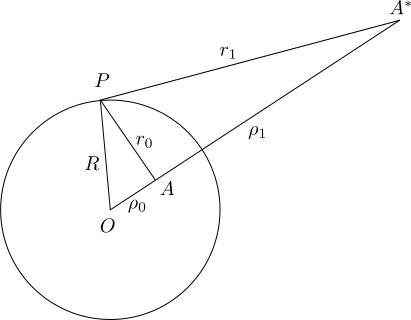
\includegraphics[width=0.4\textwidth]{figSourceFunctionCircle.pdf}
\end{wrapfigure}
\begin{minipage}[t]{0.55\textwidth}
Функция источника для круга может быть получена таким же способом, как и функция для сферы. В этом случае функцию следует искать в виде
\begin{equation}
	G = \frac{1}{2 \pi} \ln \frac{1}{r} + v
	\label{equ:equSourceFunCircle}
\end{equation}
Поместим в точку $A$ единичный заряд и отложим на радиусе, проходящем через точку $A$, такой отрезок $OA^*$, что
\begin{equation}
	\rho_0\rho_1 = R^2,
	\label{equ:SourceFunCircle1}
\end{equation}
гдe $\rho_0 = OA$, $\rho_1 = OA^*$.
Преобразование \eqref{equ:SourceFunCircle1}, ставящее в соответствие точке $A$ определённую точку $A^*$, является преобразованием обратных радиусов, а сама точка $A*$ называется \textit{сопряжённой} с точкой $A$. 
\end{minipage}\\
Докажем, что для всех точек $P$, расположенных на сфере, расстояния до $A$ и $A^*$ пропорциональны.  Для этого рассмотрим треугольники $OPA$ и $OPA^*$; они подобны, так как угол при $O$ общий, а прилежащие к нему стороны пропорциональны:
\[
	\frac{\rho_0}{R}=\frac{R}{\rho_1} \quad \mbox{или} \quad \frac{OA}{R} = \frac{R}{OA^*}
\]
Из подобия треугольников следует:
\begin{equation}
	\frac{r_0}{r_1} = \frac{\rho_0}{R} = \frac{R}{\rho_1},
	\label{equ:SourceFunCircle2}
\end{equation}
где $r_0 = \abs{\overrightarrow{AP}}$, $r_1 = \abs{\overrightarrow{A^*P}}$. Из пропорции \eqref{equ:SourceFunCircle2} получаем:
\[
	r_0 = \frac{\rho_0}{R} r_1
\]
для всех точек круга. Поэтому гармоническая функция $v = - \frac{1}{2 \pi} \ln \frac{R}{\rho_0} \frac{1}{r_1}$ на круге принимает то же значение, что и функция $\frac{1}{r_0}$. Она представляет, очевидно, потенциал заряда величины $- \frac{R}{\rho_0}$ помещённого в точку $A^*$.

Таким образом, функция 
\begin{equation}
 	G(P, A) = \frac{1}{2 \pi} \left[ \ln \frac{1}{r_0} - \ln \frac{R}{\rho_0} \frac{1}{r_1} \right],
\end{equation}
где  $\rho_0 = OA$, $r_0 = AP$, $r_1 = A^*P$, $R = OP$ -- радиус круга.
%\[
%	r_0 \cdot r_* = R^2 \Rightarrow r_* = \frac{R^2}{r_0}
%\]
%\[
%	x_* = \frac{R'}{x_0}; \quad  y_* = \frac{R^2}{y_0}; \quad  z_* = \frac{R^2}{z_0} 
%\]
%\[
%	r_{AP} = \sqrt{(x - x_0)^2 + (y - y_0)^2 + (z - z_0)^2}
%\]
%Составим функцию Грина
%\[
%	G = \frac{B}{r_{A*P}} - \frac{1}{r_{AP}}
%\]
%\[
%	r_{AP} = \sqrt{r^2 + r_0^2 - 2 r r_0 \cos \xi}
%\]
%\[
%	r_{A*P} = \sqrt{r^2 + r_*^2 - 2 r r_* \cos \xi}
%\]
%

Нетрудно убедиться в том, что определённая таким образом гармоническая функция обращается в нуль на границе
\[
	G|_{r = R} = 0
\]
%\[
%	r_{AP}|_{r = R} = \sqrt{R^2 + r_0^2 - 2 R r_0 \cos \xi}
%\]
%\[
%	r_{A*P}|_{r = R} = \sqrt{R^2 + \frac{R^4}{r_0^2} - 2 R \frac{R^2}{r_0} \cos \xi} = \frac{R}{r_0} \sqrt{r_0^2 + R^2 - 2 R r_0 \cos \xi} = \frac{R}{r_0} r_{AP}
%\]
Для решения краевой задачи надо вычислить значения $\derp{G}{n}{}$ на окружности $C$.
%\[
%	\frac{B}{\frac{R}{r_0} r_{AP}} - \frac{1}{r_{AP}} = 0; \quad B = \frac{R}{r_0}
%\]
%\begin{multline*}
%	\left. \derp{G}{u}{} \right|_{r = R} = \left.\derp{G}{r}{}\right|_{r = R} = \left[\frac{R}{r_0} \left( - \frac{1}{r_{A*P}^2} \right) \derp{r_{A*P}}{r}{} + \frac{1}{r_{AP}^2} \derp{r_{AP}}{r}{} \right] |_{r = R} = \\ = \left[ - \frac{R(r - r_* \cos \xi)}{r_0 r_{AP}^3} + \frac{1}{r_{AP}^3} (r - r_0 \cos \xi) \right]_{r = R} = \\ = \frac{-R^2 + \frac{R^3}{r_0} \cos \xi}{r_0 \frac{R^3}{r_0^3} r_{AP}^3} + \frac{R - r_0 \cos \xi}{r_{AP}^3} = \frac{1}{r_{AP}^3} \left[ - \frac{r_0^3}{R} + r_0 \cos \xi + R - r_0 \cos \xi \right]
%\end{multline*}
\[
	\left.\derp{G}{n}{}\right|_C = - \frac{1}{2 \pi R} \frac{R^2 - \rho_0}{r_0^2}.
\]
Пусть $(\rho, \theta)$ -- полярные координаты точки $P$, лежащей на окружности, а $(\rho, \theta_0)$ -- координаты точки $A$, тогда
\[
	r_0^2 = R^2 + \rho_0^2 - 2 R \rho_0 \cos (\theta - \theta_0).
\]
Подставляя в формулу 
\[
	u(\rho_0, \theta_0) = \frac{1}{2 \pi} \int\limits_C u(P) \frac{R^2 - \rho_0^2}{r_0^2} \frac{ds}{R}
\]
это выражение для $r_0$ и принимая во внимание, что 
\[
	u(P) \big|_C = f(\theta) \quad \mbox{и} \quad ds = R\, d\theta
\]
%\[
%	u(x_0, y_0, z_0) = \frac{1}{4 \pi} \iint\limits_S f(\theta) \cdot \frac{(R^2 - r_0^2)}{R(R^2 + r_0^2 - 2 R r_0 \cos \psi)^{\frac{3}{2}}}\, d \theta
%\]
%\[
%	u(r_0, \theta_0, \varphi_0) = \frac{1}{4 \pi} \int\limits_0^{2 \pi} d\varphi \int\limits_0^{\pi} f \frac{(R^2 - r_0^2) R^2 \sin \theta d \theta}{R (R^2 + r_0^2 - 2 R r_0 \cos \xi)^{\frac{3}{2}}}
%\]

%\[
%	\overline{OA} = x_0 \bar i + y_0 \bar j + z_0 \bar k = r_0 \sin \theta _0 \cos \varphi_0 \bar i + r_0 \sin \theta_0 \sin \varphi_0 \bar j + r_0 \cos \theta_0 \bar k
%\]
%\[
%	\overline{OP} = x \bar i + y \bar j + z \bar k = r (\sin \theta \cos \varphi \bar i + \sin \theta \sin \varphi %\bar j + \cos \theta \bar k)
%\]
%\[
%	\frac{\overline{OA}}{\abs{OA}} = \frac{\overline{OA}}{r_0} = \bar e (\sin \theta_0 \cos \varphi_0, \sin %\theta_0 \sin \varphi_0, \cos \theta_0)
%\]
%\[
%	\frac{\overline{OP}}{\abs{OP}} = \frac{\overline{OP}}{\bar r} = \bar e (\sin \theta \cos \varphi, \sin \theta \sin \varphi \cos \theta)
%\]

приходим для функции $u(A)$ к выражению 
\begin{equation}
	u(\rho_0, \theta_0) = \frac{1}{2 \pi} \int\limits_0^{2 \pi} \frac{R^2 - \rho_0^2}{R^2 + \rho_0^2 - 2 R \rho_0 \cos (\theta - \theta_0)} f(\theta) \, d \theta
	\label{equ:equSourceFunctionCircle}
\end{equation}
называемому \textit{интегралом Пуассона для круга}. Эта же формула с точностью до знака даёт решение внешней задачи.
